%Background and Related Work: 20%

\section{Background}
\label{sec:background}


Below mentioned are few of the works which were helpful in understanding the usage of choropleth. An example of the command-line cartography using choropleth for population density is shown in \cite {med}. Another example of the visualization of the United States election results which have an accepted standard representation of red and blue pattern in cartography is demonstrated in \cite{NYT}. An example of Zoom in feature for choropleth which helps in differentiating the visualization pattern for states and counties is shown in \cite{cmgiven}. Despite the popularity of the cartography and its variants, it is important to explore the tasks suitable for the cartography based on visualization goals. This project will be implemented using the cartography map in choropleth. The project will describe the covid cases based on per capita of each state on cartography. Terminologies In this project include: 1. Per capita category: covid cases in each state with relation to the category choose for the state. Choosing choropleth helps to better demonstrate the visualization and helps to better interpret the data. The main goal of the project is to showcase the correlation data for covid19 cases such as those based on per capita. Many of the covid19 visualization give details on cases in each county but does not compare the severity using per capita. This project focus on building the relationship between the population in each state and number of categories in covid cases in the state which will truly show the severity.

\subsection{Related Work}
\label{sec:related}


\cite{choroUn} shows an example of implementation of choropleth maps for unemployment data for different states in the United States. However, the way it is implemented, the algorithm is hard-coded for the data format and can only handle one datapoint. 

Interactive web visualization is presented in \cite{covidviz} employing a knee detection algorithm to categorize based on duration of COVID spread. While this presents a very effective data visualization and segregation, the data considered is raw data without considering per capita data and hence is subjective. Critical trends showing the live tracking of global covid cases and fatalities as shown in \cite{jhu}. This shows very detailed data split up based on states within individual countries as shown in Figure \ref{fig:JHU_Covid}. However, the drawback of this approach is the absence of any correlation data between different parameters. The user has to derive the correlation separately looking at the different plots and cartographic maps.

\begin{figure}[h]
 \centering % avoid the use of \begin{center}...\end{center} and use \centering instead (more compact)
 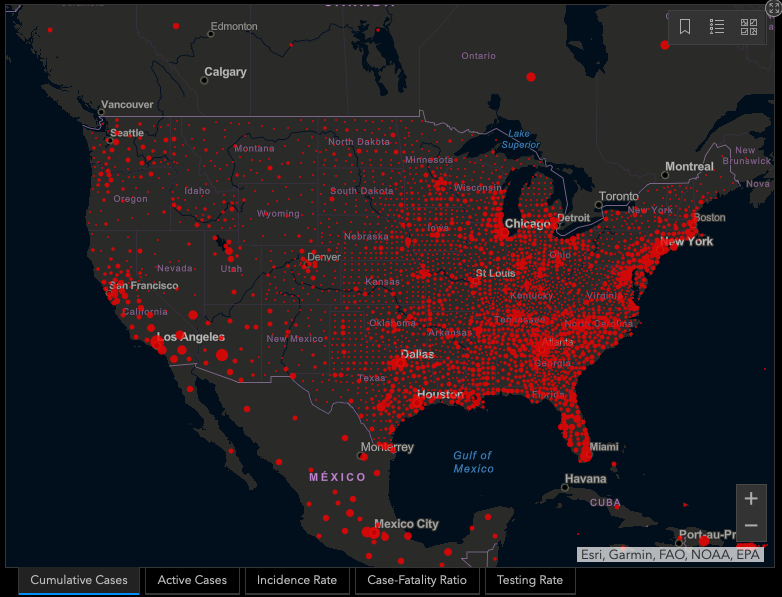
\includegraphics[width=3in]{figs/JHU_Covid.png}
 \caption{Cartographic map of Covid spread}
 \label{fig:JHU_Covid}
\end{figure}
